\documentclass[a4paper,12pt]{report}

\usepackage{cmap}
\usepackage[T2A]{fontenc}
\usepackage[utf8]{inputenc}
\usepackage[russian]{babel}
\usepackage{amsmath,amsfonts,amssymb}
\usepackage{graphicx}
\usepackage{sidecap}
\usepackage{wrapfig}
\usepackage{indentfirst}

\begin{document} 

\begin{titlepage} 

\begin{center} 

\large Федеральное государственное автономное образовательное учреждение высшего образования «Санкт-Петербургский государственный электротехнический университет «ЛЭТИ» им. В.И. Ульянова (Ленина)»\\
кафедра Вычислительной техники\\[5cm] 

\huge ОТЧЕТ\\ по лабораторной работе № 5\\[0.5cm] 
\large <<Обработка строк>>\\[3.7cm]

\begin{minipage}{1\textwidth}
    \begin{flushleft}
        \emph{Автор:} Стукен В.А.\\
        \emph{Группа:} 2307\\
        \emph{Факультет:} ФКТИ\\
        \emph{Преподаватель:} Аббас Саддам Ахмед\\
    \end{flushleft}
\end{minipage}

\vfill

Санкт-Петербург, 2022\\
{\large \LaTeX}

\end{center}
\thispagestyle{empty}
\end{titlepage}

\section*{Задание(вариант 13)}
Ввести строку символов-разделителей, а затем массив символов, который образует последовательность слов и символов-разделителей, 
находящихся в произвольном количестве до и после слов. 
Подсчитать частоты появления гласных букв в исходном массиве (набор гласных букв задается). 
Вывести результаты в виде строк из символов «*», длина каждой строки определяется значением частоты появления соответствующей гласной буквы.
\section*{Постановка задачи и описание решения}
\par

Сначала программа получает строку текста. Далее строку символов-разделителей и строку гласных.
Далее инициализируем массив, в котором будет храниться количество каждой гласной буквы в исходной строке.
Изначально заполняем данный массив нулями(функция \textit{fill-with-zeros})
Далее проходимся по строке и заполняем этот массив.
В конце выводим статистку появления гласных в исходной строке с помощью функции \textit{print-k-times}

\section*{Описание переменных-функция main}
\begin{centering}
\resizebox{14cm}{!}{
    \begin{tabular}{|l|l|l|l|}
        \hline
        \textbf{№} & \textbf{Имя переменной} & \textbf{Тип} & \textbf{Назначение}\\
        \hline
        1 & separators          &char[]& Строка символов-разделителей\\ 
        \hline
        2 &  string            & char[]  & Исходная строка текста\\ 
        \hline
        3 &  vowels     &  char[] & Строка гласных \\
        \hline
        4 & vowels-length        & int & Длина строки гласных\\ 
        \hline
        5 & vowel-count             & int[] & Массив количеств появлений каждой гласной \\
        \hline
    \end{tabular}
}
\end{centering}

\newpage
\section*{Примеры использования программы}
    \begin{figure}[h]
        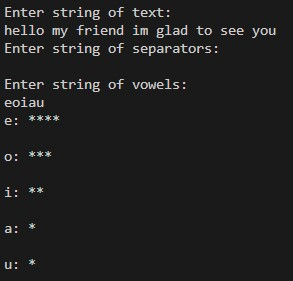
\includegraphics[width=0.5\textwidth]{ex1.jpg}
    \caption{Входные данные 1}
    \label{ris:image1}
            
        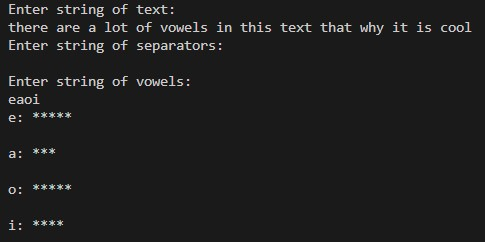
\includegraphics[width=1\textwidth]{ex2.jpg}
    \caption{Входные данные 2}
    \label{ris:image2}
    
    \end{figure}

\section*{Вывод}
В результате лабораторной работы научились работать со строками в языке Си, обрабатывать их элементы.
\end{document}